% Options for packages loaded elsewhere
\PassOptionsToPackage{unicode}{hyperref}
\PassOptionsToPackage{hyphens}{url}
\PassOptionsToPackage{dvipsnames,svgnames,x11names}{xcolor}
\documentclass[
  11pt,
  letterpaper,
]{article}
\usepackage{xcolor}
\usepackage[margin=1in]{geometry}
\usepackage{amsmath,amssymb}
\setcounter{secnumdepth}{-\maxdimen} % remove section numbering
\usepackage{iftex}
\ifPDFTeX
  \usepackage[T1]{fontenc}
  \usepackage[utf8]{inputenc}
  \usepackage{textcomp} % provide euro and other symbols
\else % if luatex or xetex
  \usepackage{unicode-math} % this also loads fontspec
  \defaultfontfeatures{Scale=MatchLowercase}
  \defaultfontfeatures[\rmfamily]{Ligatures=TeX,Scale=1}
\fi
\usepackage{lmodern}
\ifPDFTeX\else
  % xetex/luatex font selection
  \setmainfont[]{TeX Gyre Pagella}
\fi
% Use upquote if available, for straight quotes in verbatim environments
\IfFileExists{upquote.sty}{\usepackage{upquote}}{}
\IfFileExists{microtype.sty}{% use microtype if available
  \usepackage[]{microtype}
  \UseMicrotypeSet[protrusion]{basicmath} % disable protrusion for tt fonts
}{}
\makeatletter
\@ifundefined{KOMAClassName}{% if non-KOMA class
  \IfFileExists{parskip.sty}{%
    \usepackage{parskip}
  }{% else
    \setlength{\parindent}{0pt}
    \setlength{\parskip}{6pt plus 2pt minus 1pt}}
}{% if KOMA class
  \KOMAoptions{parskip=half}}
\makeatother
\usepackage{longtable,booktabs,array}
\newcounter{none} % for unnumbered tables
\usepackage{calc} % for calculating minipage widths
% Correct order of tables after \paragraph or \subparagraph
\usepackage{etoolbox}
\makeatletter
\patchcmd\longtable{\par}{\if@noskipsec\mbox{}\fi\par}{}{}
\makeatother
% Allow footnotes in longtable head/foot
\IfFileExists{footnotehyper.sty}{\usepackage{footnotehyper}}{\usepackage{footnote}}
\makesavenoteenv{longtable}
\usepackage{graphicx}
\makeatletter
\newsavebox\pandoc@box
\newcommand*\pandocbounded[1]{% scales image to fit in text height/width
  \sbox\pandoc@box{#1}%
  \Gscale@div\@tempa{\textheight}{\dimexpr\ht\pandoc@box+\dp\pandoc@box\relax}%
  \Gscale@div\@tempb{\linewidth}{\wd\pandoc@box}%
  \ifdim\@tempb\p@<\@tempa\p@\let\@tempa\@tempb\fi% select the smaller of both
  \ifdim\@tempa\p@<\p@\scalebox{\@tempa}{\usebox\pandoc@box}%
  \else\usebox{\pandoc@box}%
  \fi%
}
% Set default figure placement to htbp
\def\fps@figure{htbp}
\makeatother
\setlength{\emergencystretch}{3em} % prevent overfull lines
\providecommand{\tightlist}{%
  \setlength{\itemsep}{0pt}\setlength{\parskip}{0pt}}
\usepackage{xurl}            % allow URLs to break at any character
\usepackage{microtype}       % subtle spacing/protrusion to reduce overfull boxes
\usepackage{newunicodechar}
\newunicodechar{→}{\ensuremath{\rightarrow}}
\newunicodechar{≈}{\ensuremath{\approx}}
\newunicodechar{×}{\ensuremath{\times}}
\newunicodechar{≠}{\ensuremath{\neq}}
% Figure images: cap size so portrait photos never run off the page.
\setkeys{Gin}{width=0.72\linewidth,height=0.42\textheight,keepaspectratio}
% Last-resort horizontal slack so stubborn long lines don't overrun the margin.
\setlength{\emergencystretch}{3em}
\usepackage{bookmark}
\IfFileExists{xurl.sty}{\usepackage{xurl}}{} % add URL line breaks if available
\urlstyle{same}
% fallback for those not using the hyperref driver hyperxmp:
\makeatletter
\@ifundefined{xmpquote}{\newcommand{\xmpquote}[1]{#1}}{}
\makeatother
\hypersetup{
  colorlinks=true,
  linkcolor={blue},
  filecolor={Maroon},
  citecolor={Blue},
  urlcolor={blue},
  pdfcreator={LaTeX via pandoc}}

\title{Educational Computers in Germany in the 1980s}
\usepackage{etoolbox}
\makeatletter
\providecommand{\subtitle}[1]{% add subtitle to \maketitle
  \apptocmd{\@title}{\par {\large #1 \par}}{}{}
}
\makeatother
\subtitle{The Busch Microtronic, the Kosmos CP1, and the Philips MasterLab}
\author{Michael Wessel — translated and edited by Claude (Opus 4.8)}
\date{2026}

\begin{document}
\maketitle

{
\setcounter{tocdepth}{2}
\tableofcontents
}
\section{Educational Computers in Germany in the
1980s}\label{educational-computers-in-germany-in-the-1980s}

\subsubsection{The Busch Microtronic, the Kosmos CP1, and the Philips
MasterLab}\label{the-busch-microtronic-the-kosmos-cp1-and-the-philips-masterlab}

\emph{Original German articles by \textbf{Michael Wessel}, published in
LOAD \#10 (2024) {[}8{]} and LOAD \#11 (2025) {[}9{]} --- the magazine
of the VzEkC e.V. English translation and combined edition by
\textbf{Claude (Anthropic, Opus 4.8)}.}

\begin{quote}
This is a revised, all-in-one English edition that merges the two
original LOAD articles into a single piece. It also incorporates recent
developments (2025--2026) that were not yet available when the German
originals were written.

A print-ready PDF (US Letter) is
\href{educational-computers-in-germany-in-the-1980s.pdf}{included in
this repository}. The faithful, unmerged per-article translations are
under \href{translations/}{\texttt{translations/}}. Citations in square
brackets {[}N{]} refer to the numbered
\hyperref[references]{References}.
\end{quote}

\begin{center}\rule{0.5\linewidth}{0.5pt}\end{center}

\subsection{Introduction}\label{introduction}

In the early 1980s a new home-computer category appeared on the already
nearly saturated German market: the \textbf{educational and
experimentation computer} (\emph{Lern- und Experimentiercomputer}).
When, at the end of 1981, the first such machine for "technically
interested laypeople" appeared in German department stores --- the Busch
2090 Microtronic --- 8-bit home computers were already widespread in
Germany. Worth mentioning in particular are the representatives of the
"Trinity" (Apple II, TRS-80, Commodore PET), but also the VC-20, Atari
400 and 800, Sharp MZ-80, Sinclair ZX80 and ZX81, and the Texas
Instruments TI-99/4a. There was thus no shortage of home computers ---
so why a new device category? And what distinguishes such a computer
from a classic CPU development system or a CPU trainer?

\textbf{Predecessors.} Well-known representatives of the trainer
category include the KIM-1 (1976, 6502-based, MOS Technology) and the
MK-14 (1978, Science of Cambridge, SC/MP / INS8060 CPU). In the USA the
COSMAC ELF (RCA 1802) and the Heathkit ET-3400 trainer (Motorola 6800)
had been around since 1976, and there were various self-build projects
in the relevant computer magazines. It can be assumed, though it is not
documented, that these CPU trainers at least inspired the German
educational computers. Jörg Vallen --- who from autumn 1979 was
substantially involved in developing the Microtronic as part of his
diploma thesis --- summed up the need for a new category in the preamble
of his thesis {[}3{]}:

\begin{quote}
"At the time development of an experimentation and educational computer
began, in autumn 1979, microcomputers of this kind were hardly to be
found on the market. There were as yet no devices that enabled
non-specialists to familiarize themselves with microprocessor
technology. (\ldots) Only so-called development systems were offered by
the large semiconductor manufacturers, in order to give engineers with
appropriate training the opportunity to learn the workings of a
particular microprocessor type. Accordingly, these systems were designed
from the electronic side. The manuals and descriptions written by
specialists were (and largely still are today) incomprehensible to
non-specialists without basic knowledge."
\end{quote}

Later, Hans Vallen --- then head of the Busch company and father of Jörg
Vallen --- used the term "computer driving school" to characterize the
Microtronic {[}6{]}. So what defines an educational and experimentation
computer? Four points stand out:

\begin{itemize}
\tightlist
\item
  \textbf{Educational focus.} The target group is "interested
  laypeople", and children and teenagers in particular. The manuals
  especially must therefore be designed with a certain didactic standard
  --- many classic CPU trainers are inadequate here, and many were only
  available as kits. The educational angle surely also convinced some
  parents that an educational computer was a better buy than a BASIC
  home computer used mainly for games (which would moreover compete for
  the family television set).
\item
  \textbf{Experimentation focus.} The aim is not only to learn
  programming, but also to combine it with experiments on electronic
  circuits ("physical computing"). General-purpose input/output ports
  (GPIOs) are therefore required --- ideally robust against miswiring,
  to enable "worry-free experimentation". Today one would use an Arduino
  for this; in contrast, the educational computers of the 1980s were
  complete systems that needed no additional "PC" for programming.
\item
  \textbf{Cost.} A "real" BASIC home computer was an expensive barrier
  to entry. With the exception of the Sinclair ZX80/81, these still cost
  around DM 700 and up, plus peripherals, software and books --- and
  that only changed with the price collapse of 1984. By contrast, the
  Microtronic was advertised in 1981 {[}7{]} at DM 379, falling to DM
  299 by 1984. For comparison: a VC-20 still cost DM 798 at the end of
  1981 --- a full week\textquotesingle s salary, given an average German
  annual income of DM 30,900.
\item
  \textbf{Availability.} CPU trainers were hard for ordinary consumers
  to obtain --- often kit-only and known only to readers of electronics
  and amateur-radio magazines. Department stores did not carry them. The
  educational computers, by contrast, were sold where families actually
  shopped.
\end{itemize}

German educational computers are a fascinating and magnificent piece of
technical history that did not exist in this form in other countries.

\subsection{How this article is
structured}\label{how-this-article-is-structured}

This article presents three representatives of the German
educational/experimentation category, \textbf{in historical order}, each
in its own section:

\begin{enumerate}
\def\labelenumi{\arabic{enumi}.}
\tightlist
\item
  the \textbf{Busch Microtronic} (1981) --- a 4-bit TMS1600-based
  machine with a remarkably terse and powerful interpreted instruction
  set;
\item
  the \textbf{Kosmos CP1} (1983) --- an 8-bit Intel 8049-based decimal
  von-Neumann machine with an unusually rich set of GPIOs;
\item
  the \textbf{Philips MasterLab} (1983) --- an INS8070 (SC/MP III)-based
  machine that is, of the three, the only "real" CPU trainer.
\end{enumerate}

A comparison and an overall conclusion follow at the end.

\begin{center}\rule{0.5\linewidth}{0.5pt}\end{center}

\subsection{1. The Busch Microtronic
(1981)}\label{1-the-busch-microtronic-1981}

\pandocbounded{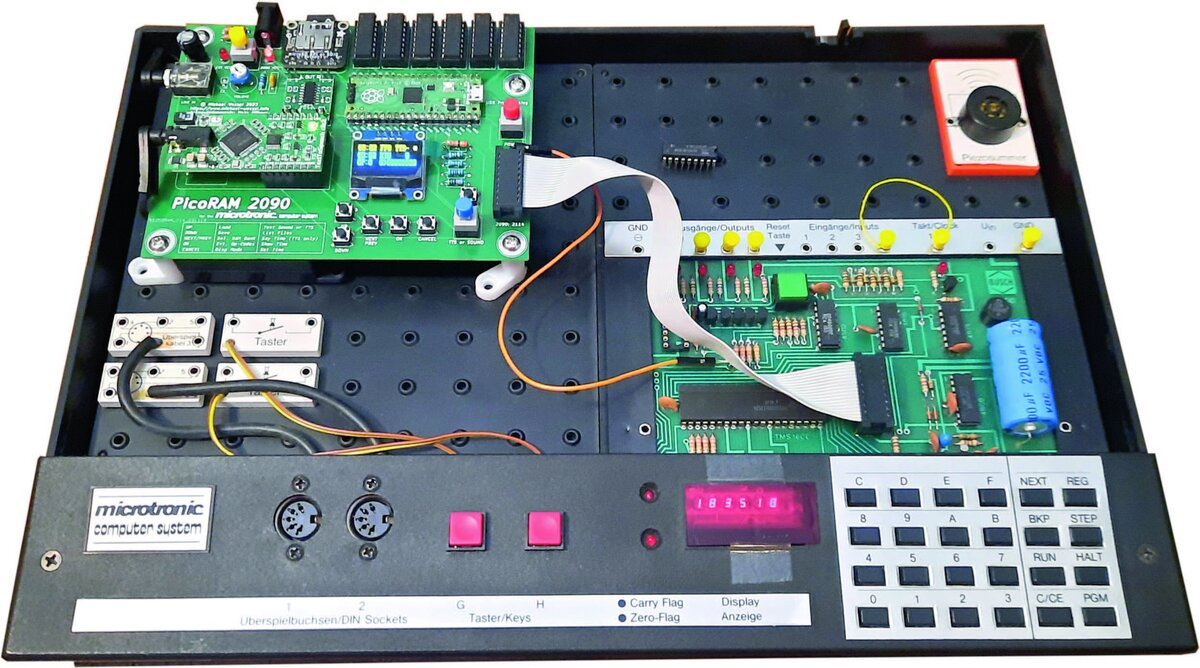
\includegraphics[keepaspectratio,alt={Busch Microtronic with PicoRAM 2090}]{images/microtronic-picoram.jpg}}

\emph{Figure 1. The Busch Microtronic, shown with the modern PicoRAM
2090 SD-card expansion {[}14{]}.}

Busch electronics kits had been available in Germany since 1976; until
October 1981 they were distributed under the name "ELOtronic" by the
Franzis publishing house. The Microtronic was conceived as the
complement and flagship of the Busch electronics-kit series. Its
appearance can be called elegant and high-quality --- the case and build
make a sturdy impression, the smoked-glass cover looks professional, and
the keyboard allows even longer program entry without frustration, in no
way inferior to the TI calculator keyboards of the era (TI-30,
TI-58/59).

The heart of the Microtronic is a mask-programmed \textbf{TMS1600 4-bit
microcontroller, clocked at 500 kHz}. The firmware contains the
operating system and an interpreter for a virtual machine language. The
Microtronic is therefore programmed not in TMS1600 machine language, but
in a higher-level Microtronic machine language --- easier to learn, and
offering very powerful instructions, for example for multiplication and
division.

\textbf{Development.} Development work began in autumn 1979. The
hardware and operating system were carried out, to
Busch\textquotesingle s specifications, by the company "MRT -- Mess- und
Regeltechnik" in Kaisersbach (now insolvent); Jörg Vallen worked there
directly as part of his thesis and made essential contributions. Texas
Instruments in Freising took over production of the mask-programmed
TMS1600. The instruction set, originally 20 instructions, was expanded
to 41 in the second development phase --- again with Jörg Vallen
instrumental: as the first application developer, following "eat your
own dog food!", he identified deficits and further desirable
instructions (random numbers, multiplication, division). The thesis
{[}3{]} also reveals that originally a TMS1xxx development system with
EPROMs was used (possibly an HE-2), and that the finished operating
system was handed over to TI "on a floppy disk". As program memory, the
developers connected a 2114 SRAM chip via the TMS1600 "GPIO port" ---
although the TMS family, as a "computer on a chip", provides for no
external memory at all. The 1 KByte of 4-bit words of the 2114 is used
as program memory; the SRAM on the TMS1600 holds the 32 4-bit
Microtronic registers and monitor variables.

\textbf{Harvard architecture.} The program memory comprises 256
addresses (0x00--0xFF), and each instruction is three nibbles (12 bits).
Program and data memory are strictly separated: as program-writable data
memory the Microtronic offers exclusively the registers (plus
immediate-addressing instructions). Of the 32 registers, 16 are working
and the rest background registers, swappable in banks of 8 so that data
can be transferred between foreground and background. All
logical-arithmetic operations and data must fit into these 32 4-bit
registers. The hexadecimal number system is used; the hex keypad has
eight function keys, and the display is a six-digit seven-segment
"bubble LED" display (as in old TI calculators), with two LEDs for the
carry and zero flags. A green reset key is on the board --- and the
program memory survives a reset. A DIL expansion socket connects the
"2095" cassette interface; four digital outputs, four digital inputs,
and a 1 Hz clock signal are brought out as plug sockets.

\textbf{Built-in programs.} On power-up the monitor shows "00 000" ---
address on the left, instruction on the right (both hex). RUN starts at
the current address; the monitor offers single-step (STEP) and
breakpoints (BRK), and register inspection/editing via REG. PGM calls
built-in programs: cassette load/save (PGM 1/2), the NIM game (PGM 7),
clear memory (PGM 5), self-test (PGM 0), and display/set the
(non-battery-backed) real-time clock (PGM 3/4). PGM 6 fills memory with
NOPs.

\textbf{Instruction set.} The instruction set is terse, pragmatic and
must be called extremely well-designed. It includes instructions to
control the display (showing up to six consecutive registers), keyboard
input, GPIO, random numbers, time-of-day queries, logical-arithmetic and
bitwise operations, and hex/decimal conversion. Most operations can be
performed equally in all registers --- the set is very orthogonal,
similar to modern RISC CPUs. The carry flag combines arbitrary 4-bit
registers into larger ones, so addition and subtraction can run up to 64
bits (division is limited to four, multiplication to six digits). Set
flags trigger conditional jumps. Subroutines exist (CALL/RET) but cannot
be nested. The biggest shortcoming is that only two addressing modes are
supported (immediate and register-direct); jump targets are always
immediate, so they cannot be computed --- indirect and computed jumps,
and thus recursion, require relatively complicated trickery. (The author
nonetheless succeeded in implementing a recursive Towers of Hanoi on the
Microtronic {[}10{]}.) None of this harms the overall impression of a
universal computer; the manual programs are throughout quite general ---
the NIM game actually computes the optimal winning strategy.
Interpreting the instruction set costs time, though: a typical maximum
is about 114 instructions per second, dropping to about 40 with the
display on; some programs (e.g. dividing 9999 by 1) take up to 8
seconds.

\textbf{Manual.} The two-volume manual {[}1{]}, written by Jörg Vallen
and lovingly illustrated with the "Buschi" mascot, is didactically
excellent: Part 1 introduces the Microtronic, Part 2 covers more complex
programs, circuits and experiments with additional Busch kits.
Highlights include a moon-landing game, a perpetual calendar, biorhythm
calculation, a calculator, tic-tac-toe and sine computation; the
electronics section covers timers, tone/music generators, model-railway
control, a frequency counter and a reaction-time meter. An English
translation of this classic manual (Part 1) is now underway {[}2{]},
making it accessible to a wider, non-German-speaking audience. A clever
\textbf{trick} works around the low \textasciitilde3--4 Hz GPIO sampling
rate: input 4 clocks the firmware\textquotesingle s background real-time
clock, which can register frequencies up to 60 Hz, so externally
generated pulses are counted automatically and read out via the
"get-time" instruction (F06).

\textbf{Extensions, old and new.} The original "2095" cassette interface
is leisurely (a full dump takes \textasciitilde220 s ≈ 14 baud); the
"2092 special interface" doubles the GPIOs and adds relay-driving
transistors (e.g. for Fischertechnik robots). There is no dedicated
expansion bus --- everything goes through the normal GPIOs. Modern
extensions by the author include an Arduino-based speech synthesizer and
a
\href{https://github.com/lambdamikel/microtronic-2095-arduino-emulator}{2095
SD-card emulator} {[}15{]} (building on Martin Sauter\textquotesingle s
2017 protocol decode), and especially
\href{https://github.com/lambdamikel/picoram2090}{\textbf{PicoRAM 2090}}
{[}14{]}, a Raspberry Pico-based RAM emulator with SD card that replaces
the 2114, adds bank-switched memory expansion and an extensive I/O
expansion (speech, sound, OLED text/graphics, battery-backed clock). It
is addressed through 64 "redundant", ineffective instructions (such as
\texttt{MOV\ \textless{}x\textgreater{}\ →\ \textless{}x\textgreater{}},
a NOP-like register-to-self copy) that never occur in normal programs;
PicoRAM repurposes them as new side effects. PicoRAM 2090 won the
RetroChallenge 2023/10 Grand Prize. A range of emulators also exists ---
the first written by the author in 1985 on a Schneider CPC 464 in BASIC;
a \href{https://freeshell.de/~d01c/micsim_0.1.0.tar.xz}{C/Linux
emulator} by Ingo D. Rullhusen {[}32{]}; a
\href{https://download.cnet.com/2090-emulator/3000-2072_4-47314.html}{Macintosh
app} by Stephan Kleinert {[}33{]}; and
\href{https://github.com/lambdamikel/Busch-2090}{Arduino-based hardware
emulators} {[}13{]} from 2016 onward, including the "Microtronic 2nd /
Next Generation" re-editions built into a Busch "2070" console (Hackaday
"Reinvented Retro Contest" winner, 2021).

\pandocbounded{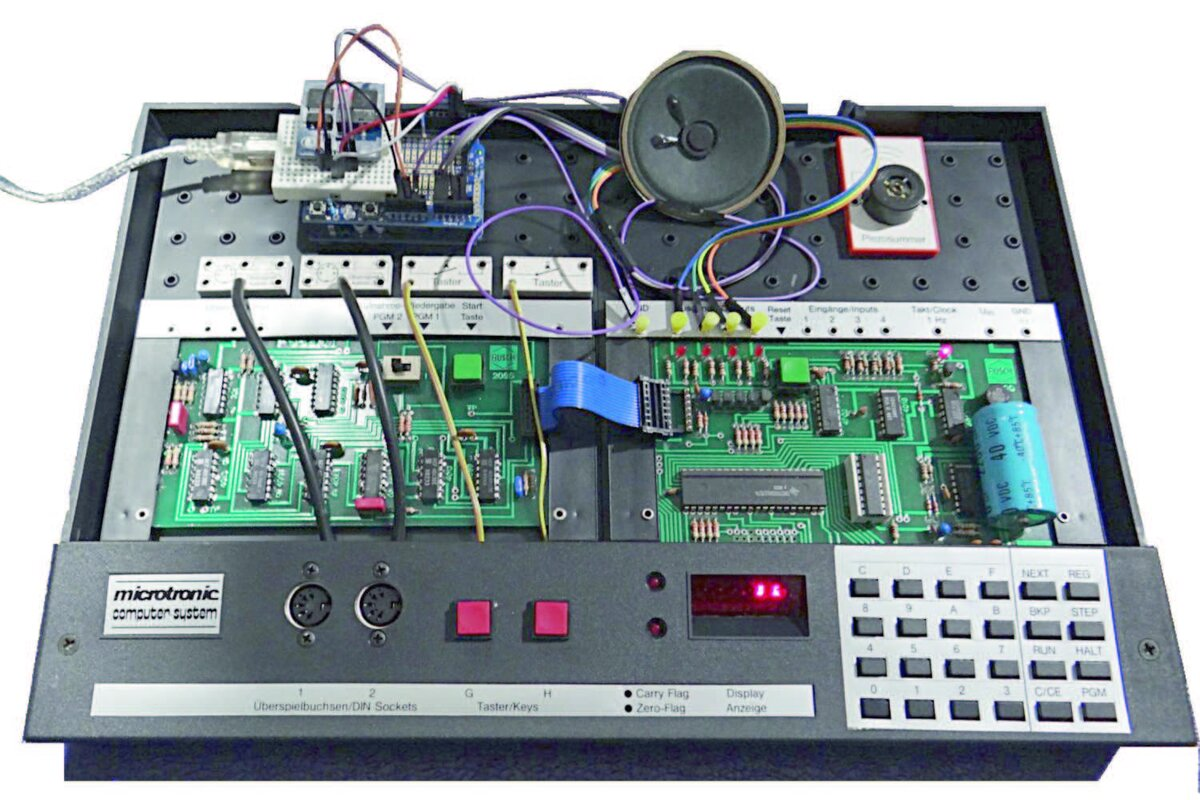
\includegraphics[keepaspectratio,alt={Busch Microtronic with 2095 cassette interface and speech synthesizer}]{images/microtronic-2095.jpg}}

\emph{Figure 2. The Busch Microtronic with the original 2095 cassette
interface and a DIY speech synthesizer.}

\textbf{Recent developments (2025--2026).} The author has also used the
Microtronic as the brain of larger systems: a recursive
\href{https://github.com/lambdamikel/towers-of-hanoi}{Towers of Hanoi}
{[}10{]} solver drives a physical pan/tilt \textbf{Hanoi robot} and,
most recently, animates the solution on a \textbf{64×32 RGB LED matrix}
--- via a microcontroller that reads the Microtronic\textquotesingle s
moves over a simple 4-bit GPIO protocol (a video of the recursive solver
running on the Microtronic is available {[}37{]}). And, most
significantly of all, the original Microtronic firmware ROM was finally
recovered and brought back to life on new hardware: the
\href{https://github.com/lambdamikel/microtronic-phoenix}{\textbf{Microtronic
Phoenix}} {[}16{]}, described in the appendix.

\textbf{Björn Rathje\textquotesingle s projects.} The most ambitious and
impressive \emph{contemporary software} projects for the Microtronic ---
the author\textquotesingle s own Towers of Hanoi notwithstanding ;-) ---
come from \href{https://github.com/rab-berlin}{\textbf{Björn Rathje}}
{[}20{]}. Working purely in the Microtronic\textquotesingle s tiny
256-instruction machine language, he has produced a remarkable body of
work that pushes the little 4-bit machine far beyond what its 1981
manuals imagined:

\begin{itemize}
\tightlist
\item
  \href{https://github.com/rab-berlin/Monarch2090}{\textbf{Monarch2090}}
  {[}21{]} --- a faithful simulation of the legendary \emph{Rotomat
  Monarch} (1972) slot machine on the Microtronic; the standout piece,
  and the most elaborate.
\item
  \href{https://github.com/rab-berlin/Kniffel2090}{\textbf{Kniffel2090}}
  --- Yahtzee (Kniffel) for the Microtronic.
\item
  \href{https://github.com/rab-berlin/Mensch2090}{\textbf{Mensch2090}}
  --- "Mensch ärgere dich nicht" (the German Ludo / "Sorry!"-style board
  game).
\item
  \href{https://github.com/rab-berlin/Invaders2090}{\textbf{Invaders2090}}
  --- Space Invaders on the Microtronic.
\item
  \href{https://github.com/rab-berlin/Life2090}{\textbf{Life2090}} ---
  Conway\textquotesingle s Game of Life.
\item
  \href{https://github.com/rab-berlin/BerlinUhr2090}{\textbf{BerlinUhr2090}}
  --- the Berlin "set-theory clock" (Mengenlehre-Uhr) rendered on the
  Microtronic.
\item
  \href{https://github.com/rab-berlin/Film2090}{\textbf{Film2090}} ---
  "the Microtronic goes to Hollywood": a playful animation/film project.
\item
  \href{https://github.com/rab-berlin/ESP2090}{\textbf{ESP2090}} --- a
  modern take pairing the Microtronic world with an ESP32 and
  MicroPython.
\end{itemize}

That a 4-bit, 500 kHz machine with 1 KB of program memory can host a
slot-machine simulation, several board and arcade games, and Game of
Life is a testament both to the elegance of the Microtronic instruction
set and to Rathje\textquotesingle s ingenuity.

\begin{center}\rule{0.5\linewidth}{0.5pt}\end{center}

\subsection{2. The Kosmos CP1 (1983)}\label{2-the-kosmos-cp1-1983}

\pandocbounded{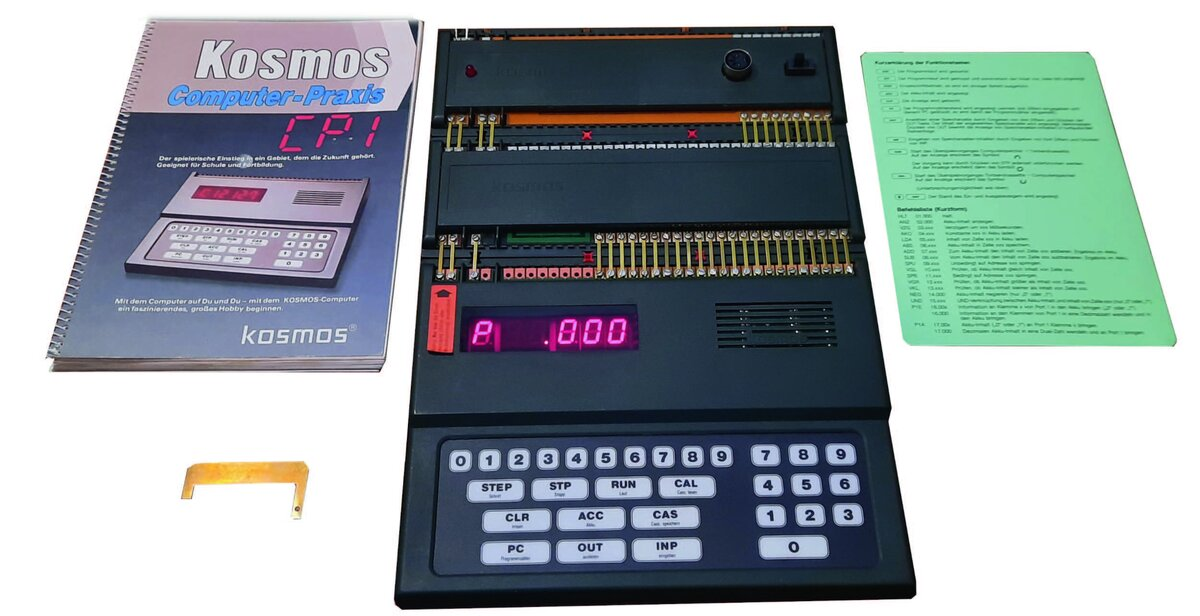
\includegraphics[keepaspectratio,alt={Kosmos CP1 with manual and quick-reference card}]{images/cp1.jpg}}

\emph{Figure 3. The Kosmos CP1, with its spiral-bound manual and the
green quick-reference card.}

The Kosmos CP1 was released in 1983 at an introductory price of DM 198,
as a complement to Kosmos electronics kits (for example the "Elektronik
Labor" sets): a Kosmos breadboard with the typical clamp contacts can be
attached to it, and cables for the screw terminals at the back screw on
directly. Its appearance is modern --- the membrane keyboard and the
large six-digit seven-segment display catch the eye, and it is
immediately clear that exclusively the \textbf{decimal} number system is
used (the hex digits A--F are nowhere to be found; the digit keys are
even duplicated). The case is shapely but the build quality does not
fully convince (thin plastic, a thick-cardboard base, and these days a
strong flux smell). The membrane keyboard does not allow "blind" typing
--- there is no haptic pressure point --- and the duplicated digit keys
are, in the author\textquotesingle s opinion, a waste of space; the CAL
key sits unfortunately close to INP, causing frequent accidental
activations.

\textbf{Processor.} The heart of the CP1 is a mask-programmed
\textbf{Intel 8049}, accompanied by an 8155 serving as 2 KByte 8-bit
SRAM and for I/O. (Some units use the non-mask-programmed 8749 with an
external EPROM instead --- possibly early versions.) The 8049 is clocked
at 6 MHz. Notably, the foreword of the manual {[}4{]} was written by
Prof. Karl Steinbuch, a prominent information-processing professor at
the University of Karlsruhe, though his influence on the design is not
documented. The CP1 is not programmed in the
microcontroller\textquotesingle s machine language (MCS-48) but in a
virtual machine language executed by an interpreter; the 2 KB firmware
contains the interpreter, the monitor and a few built-in programs.

\textbf{Architecture.} The CP1 is laid out as a strict, almost academic
\textbf{decimal von-Neumann machine}. The only register is an
accumulator; all operations to and from memory must pass through this
"von-Neumann bottleneck". The base version offers 128 memory cells
(program and data); the CP3 expansion raises this to 256. All data,
instructions and addresses are encoded in decimal. Cells hold values
from "00.000" to "24.255": for a cell "xy.abc", "xy" is the instruction
code (01.--24.) and "abc" the operand or address (0--255); data cells
use "00.abc". A separate decimal 8-bit I/O pointer (EAZ), shown via "9
OUT", is used for entering and inspecting cells (entries via "IN"/Enter
auto-increment it). There is no breakpoint facility --- one inserts HALT
manually. The decimal scheme and the cumbersome "9 OUT" mechanism are
ergonomically inferior to what hexadecimal would have afforded.

\textbf{Instruction set.} Instructions exist to display and delay, to
load the accumulator with a constant or a cell and store it back, and to
add/subtract a cell. An "implicit" flag is set by comparing the
accumulator with a cell (equal/less/greater), after which a conditional
(or unconditional) jump can run. A binary (0/1) accumulator can be
negated and AND-ed with a binary cell; there are no bitwise operations.
A loaded cell brings in both the operand "abc" \emph{and} the opcode
"xy."; performing arithmetic on a cell that actually holds an
instruction (xy. ≠ 00) aborts the program with "F 002".

\textbf{Strengths and weaknesses.} A real strength is \textbf{indirect
loading/storing} of the accumulator --- like pointer variables in C ---
enabling lists, stacks and arrays, plus \textbf{indirect jumps} that
make return stacks, nested subroutine calls, recursion, and even
self-modifying and relocating programs possible. (Amusingly, the
manual\textquotesingle s relocation program only works in restricted
cases --- because of indirect addressing, program relocation is in
general undecidable.) Against this, much is missed: I/O is limited (the
display only shows the accumulator; the keyboard cannot be read by
programs --- external metal-bracket buttons serve instead), and there
are no multiply/divide, random-number, or bitwise instructions. The
accumulator must not over- or underflow (\textgreater255 or \textless0
aborts with "F 006", and there is no carry flag) --- but here the
decimal system becomes a stroke of genius: "greater than 99" comparisons
let several cells be combined into arbitrarily wide registers, since 2 ×
99 \textless{} 255. The instruction set is not terse: the strict
von-Neumann model means almost every operation is load → manipulate →
store, tripling the instruction count and quickly exhausting memory. The
CP1 thus illustrates the von-Neumann bottleneck excellently (though the
manual does not address this). It is, however, considerably faster than
the Microtronic --- the interpreter runs at about \textbf{3200
instructions/second}, nearly 30× the Microtronic --- which matters for
the GPIOs.

\textbf{GPIOs and extensions.} The CP1\textquotesingle s large number of
GPIOs is a clear strength: the base version already has an 8-bit
input/output plus an 8-bit output, and the CP3 expansion adds a second
8-bit input/output and two further outputs (8 and 6 bits). Unlike the
Microtronic, the CP1 has a dedicated expansion bus: the CP2 cassette
interface, the CP3 memory/port expansion, the CP4 relay module (model
railways, Fischertechnik robots) and the CP5 (eight LEDs + amplifiers on
output 2, eight slide switches on input 1) can all be combined. The
manual {[}4{]} is lovingly and didactically high-quality, using the
"Computron" character to carry out the CPU operations; its programs
resemble the Microtronic\textquotesingle s (NIM, moon landing, dice,
Senso, number guessing) and kit-based projects (timers, reaction
testers, blinking lights, tone generators, alarms, model-railway
control). Compared with the Microtronic, some programs are less general
--- e.g. the CP1\textquotesingle s NIM is hard-coded for 15 sticks / 3
removable and uses external buttons for input, since the keyboard cannot
be read by programs. Both software and hardware (Arduino-based)
emulations and re-implementations exist; since the firmware is available
and the parts are standard, faithful re-implementations are easy (e.g.
\href{https://www.g-heinrichs.de/wordpress/index.php/informatik/minipc/}{MiniPC}
{[}26{]} emulates the 8049 and runs the original firmware, while a
\href{https://sourceforge.net/projects/cp1-sim/}{Java-based emulator}
{[}27{]} reimplements the virtual machine directly), and an
\href{https://github.com/asig/kosmos_tape_emulator}{Arduino-based CP2
cassette emulator} {[}23{]} has been developed. Further background on
the CP1 is collected at the
\href{http://www.8bit-homecomputermuseum.at/computer/kosmos_computer_praxis_cp1.html}{8-bit
Home Computer Museum} {[}28{]}.

\textbf{Recent developments (2025--2026).} The same recursive Towers of
Hanoi also runs on the CP1, which can likewise drive the 64×32
LED-matrix renderer. To make writing and loading CP1 programs painless,
the author built a small
\href{https://github.com/lambdamikel/kosmos-cp1-devel-toolchain}{\textbf{CP1
development toolchain}} {[}11{]}: a real assembler (mnemonics, labels),
and --- after digitizing a genuine CP2 cassette save and
reverse-engineering the previously undocumented CP1/CP2 FSK tape format
--- a tool that turns a program into a \textbf{cassette WAV} you simply
play into the CP2, so programs load without any hand-keying (a video of
the recursive Towers of Hanoi running on the CP1 is available {[}38{]}).
This builds on a lively CP1 community --- the
\href{https://github.com/asig/kosmos-cp1}{asig/kosmos-cp1} {[}22{]}
emulator (with an integrated assembler and an SD-card tape emulator),
the
\href{https://github.com/RalphBln/kosmos-cp1-arduino-cassette-emulator}{RalphBln
cassette emulator} {[}24{]}, and the
\href{https://github.com/moosy/kosmos-cp1-toolchain}{moosy CP1
toolchain} {[}25{]} are all valuable companions.

\begin{center}\rule{0.5\linewidth}{0.5pt}\end{center}

\subsection{3. The Philips MasterLab
(1983)}\label{3-the-philips-masterlab-1983}

\pandocbounded{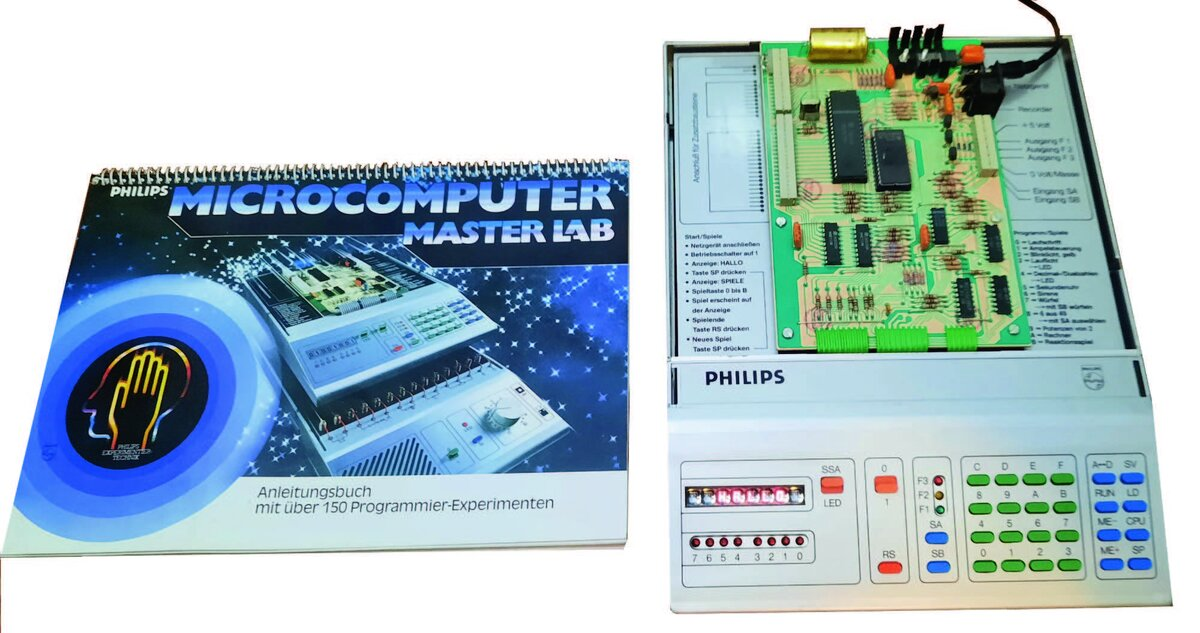
\includegraphics[keepaspectratio,alt={Philips MasterLab and its manual}]{images/masterlab.jpg}}

\emph{Figure 4. The Philips MasterLab and its "Microcomputer Master Lab"
manual.}

Philips was at the time probably the second-largest supplier of
experimentation kits on the German market, behind the leader Kosmos. In
1983 the MasterLab came out under the Philips label for DM 449.00, as
part of the new "6000" ("ABC") series; from 1984 Philips withdrew from
the kit market and the series continued under the Schuco name (the
takeover by the Mangold Group --- Schuco, Trix, GAMA --- had been
decided in 1982). The 6000 kits, and thus the MasterLab, had been
developed by Philips\textquotesingle s educational-materials department
together with the "Institut für Lehrerfortbildung" (Institute for
Teacher Training) in Hamburg --- in particular by Mr. Erhard Meyer,
author of the manual {[}5{]}, whose initials "E.M." also appear in the
firmware EPROM ("COPYRIGHT 1982,1983 (C) GAMA, E.M., \ldots"). What
seems certain is that the MasterLab\textquotesingle s birthplace lies in
Hamburg; more on its origins is collected on the
\href{https://norbert.old.no/kits/6400/6400.html}{Philips/Schuco 6400
information page} {[}30{]}.

\textbf{External attributes.} The MasterLab is a feast for the eyes ---
a shapely silver case with a transparent Plexiglas hood, colorful keys,
and a seven-segment LED display of \textbf{eight} digits instead of six.
A row of eight LEDs sits below the display, with three further LEDs (F1,
F2, F3) and two input buttons (SA, SB); an SSA/LED switch toggles the
display between seven-segment mode and the eight LEDs (driven by the
middle digit\textquotesingle s 7+1 segments). It even has an on/off
switch and a reset button --- neither of which the Microtronic or CP1
has --- plus eight function keys for the monitor.

\textbf{An unusual CPU.} The board carries an \textbf{INS8070 (SC/MP
III) CPU clocked at 4 MHz}. As in the Microtronic, a 2114 SRAM (here
doubled, for 8 bits) provides 1 KB at 0x1000--0x13FF, with the firmware
in a 4 KB (2732) EPROM up to 0x0FFF. Unlike the Microtronic and CP1,
which run an interpreted higher-level language, the MasterLab is
programmed \textbf{directly in INS8070 machine language} --- it is
therefore more a classic CPU trainer than an "educational computer", and
consequently far faster: the author measured \textbf{147,050
instructions/second}, making it roughly 1,290× the Microtronic and about
46× the CP1 (see the benchmark below). On power-up the monitor shows a
friendly "HALLO" --- making clear the display is good for more than hex;
in fact every segment of every digit can be addressed individually (as
the scrolling-text demo shows).

\textbf{Button-controlled GPIOs.} The buttons SA, SB and LEDs F1, F2, F3
are the GPIOs, brought out as a header and transistor-buffered --- so
the MasterLab offers only three digital outputs and two digital inputs
(somewhat meager). Their connection is elegant, though: they are
controlled \textbf{directly by the INS8070\textquotesingle s flag/status
register}, needing no firmware support, and SA/SB can even trigger
interrupts --- making them about two orders of magnitude faster than the
CP1\textquotesingle s. Unlike the others, the MasterLab has a built-in
cassette interface, realized almost entirely in software: the fast I/O
lets the CPU both generate the 1/2 kHz cassette tones and read them back
via the SB input, observing the pulses directly in the status register.
An expansion bus on the left brings out address, data and control buses
(a RAM expansion would be easy); expansion boards were apparently
envisioned but never released.

\textbf{Firmware, manual and capabilities.} The firmware holds demo
programs (siren, lottery numbers, calculator, scrolling text, digital
clock, traffic-light control on the F-LEDs, dice, \ldots), started via
the SP key; the monitor resembles comparable trainers (e.g. the
Multitech MPF-1), with A/D for address/data, ME+/ME- to step the
address, SV/LD for cassette, and CPU to inspect/modify registers ("CPU
6" = accumulator, "CPU 0" = PC). Breakpoints and single-step are absent,
but a HALT can be inserted manually. The manual {[}5{]} is a deep,
comprehensive introduction to INS8070 programming --- the CPU even
offers 16-bit operations (the multiply combines A and E into a 16-bit
register multiplied by the 16-bit T register, giving a 32-bit A,E,T
result; a divide exists too), a stack pointer, two pointer registers
(SP1, SP2) for indexed addressing, interrupts, and a wealth of
addressing modes (immediate, absolute, implied, direct, indirect,
indexed, relative). Firmware CALL routines ease programming (display
control, 2-/4-digit hex input, decimal/hex conversion). The biggest
shortcoming is the limited experimentation capability --- the manual
only demonstrates a loudspeaker, a lamp and a simple photoresistor light
barrier; more GPIOs would have helped. The direct, firmware-free
coupling of the GPIOs to the CPU is nonetheless brilliant. The learning
material is far more complex, comprehensive and technical than the
others\textquotesingle{} --- a steeper curve, clearly aimed at adults /
teacher training, and presented bone-dry --- but the MasterLab is the
only one offering a complete, realistic, practical path to
microprocessor programming.

\pandocbounded{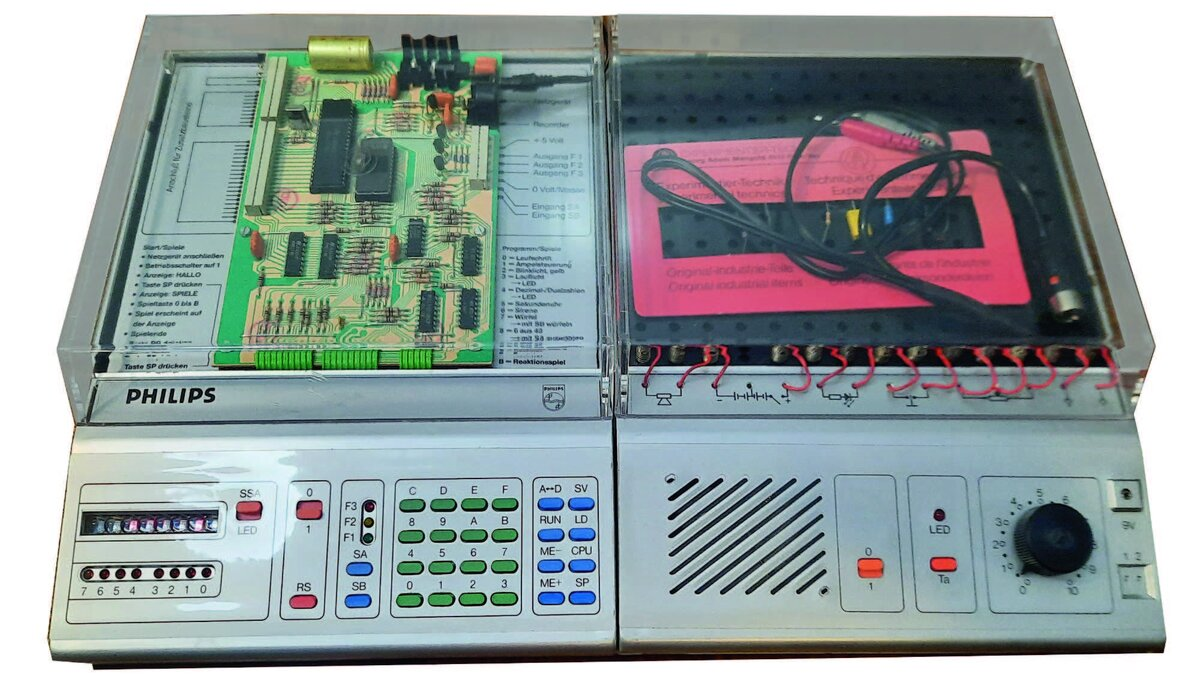
\includegraphics[keepaspectratio,alt={Philips MasterLab with an attached experiment box}]{images/masterlab-expbox.jpg}}

\emph{Figure 5. The Philips MasterLab with an attached experiment box.}

\textbf{Recent developments (2025--2026).} Several projects have since
appeared. Thorsten Brehm ("MacFly") built a complete
\href{https://github.com/ThorstenBr/MasterLab-MC6400}{MasterLab
\textbf{emulator}} {[}29{]} in JavaScript/HTML-CSS (November 2024),
playable online --- the emulator used as a reference while developing
the vector display below. And the author built a
\href{https://github.com/lambdamikel/philips-mc6400-vector-graphics}{\textbf{vector-graphics
display}} {[}12{]} for the MasterLab: a program drives an X-Y
oscilloscope to show a rotating 3-D wireframe (cube, torus, sphere) via
a homemade R-2R DAC on the expansion bus --- turning the
INS8070\textquotesingle s speed and the expansion bus into a small
vector-graphics engine.

Crucially, the perennial problem of \emph{getting programs into the
machine} now has a modern solution:
\href{https://github.com/lambdamikel/picoram-ultimate}{\textbf{PicoRAM
Ultimate}} {[}31{]}, a Raspberry Pi Pico--based SD-card RAM emulator for
the MasterLab (a sibling of the Microtronic\textquotesingle s PicoRAM
2090). It plugs directly into the MasterLab\textquotesingle s two 2114
SRAM sockets via a ribbon cable and stands in for the
machine\textquotesingle s RAM, loading and saving complete program
images directly from an SD card. That turns the old chore of hand-keying
--- or waiting on the slow software cassette --- into a file exchange: a
demo such as the vector-graphics engine above can be dropped onto the SD
card on a PC and loaded into the MasterLab in seconds, and programs can
be archived and shared as ordinary files. PicoRAM Ultimate did not exist
when the original article was written; today it is the most convenient
way to develop for, and experiment with, the MasterLab.

\pandocbounded{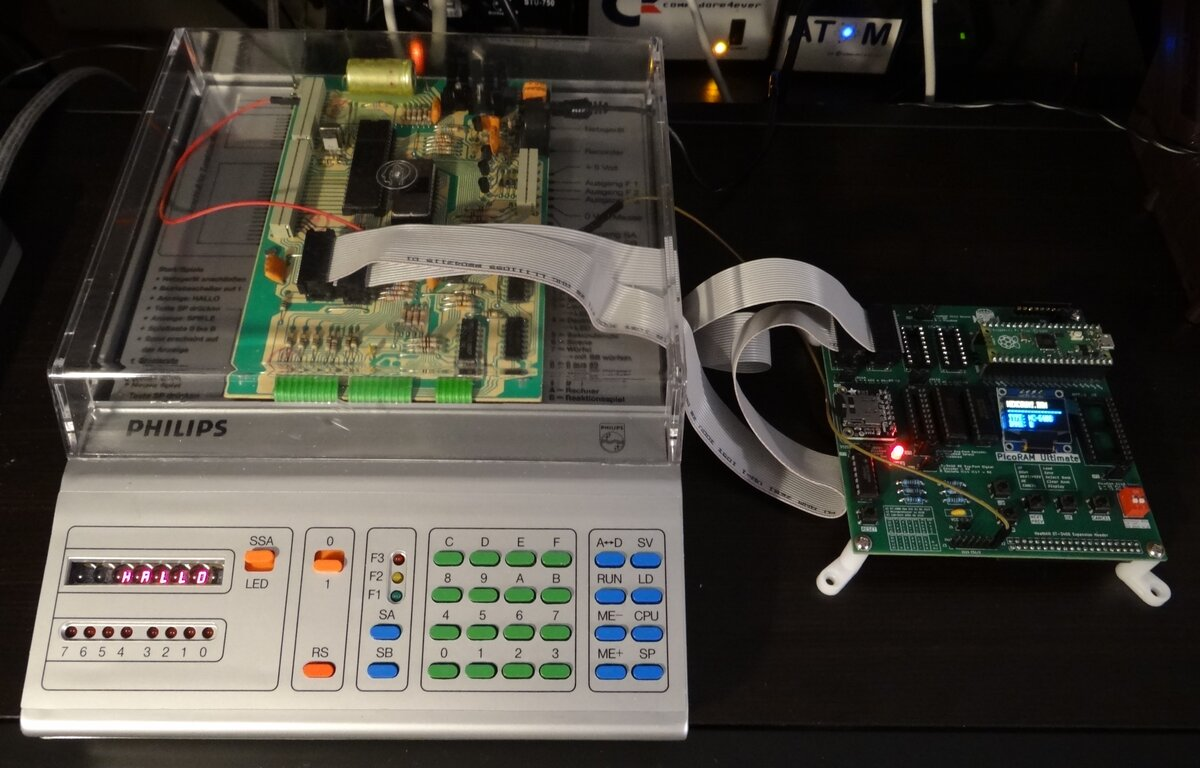
\includegraphics[keepaspectratio,alt={PicoRAM Ultimate connected to the Philips MasterLab}]{images/picoram-ultimate-masterlab.jpg}}

\emph{Figure 6. PicoRAM Ultimate (right) connected to the Philips
MasterLab --- it plugs directly into the machine\textquotesingle s two
2114 SRAM sockets via the ribbon cable; the MasterLab\textquotesingle s
display shows its "HALLO" power-up greeting {[}31{]}.}

\begin{center}\rule{0.5\linewidth}{0.5pt}\end{center}

\subsection{Comparison and conclusion}\label{comparison-and-conclusion}

\subsubsection{Speed: a measured
benchmark}\label{speed-a-measured-benchmark}

How fast are these machines, really? The author measured each one with
the same simple benchmark --- a program that toggles a GPIO output as
fast as possible --- and counted the resulting \textbf{instructions per
second (ips)}. The differences are dramatic, and follow directly from
the architectures: the Microtronic and CP1 \emph{interpret} a virtual
machine language (and the Microtronic is only 4-bit at 500 kHz), whereas
the MasterLab runs INS8070 \textbf{native machine code} at 4 MHz.

{\def\LTcaptype{none} % do not increment counter
\begin{longtable}[]{@{}lllrr@{}}
\toprule\noalign{}
Computer (CPU) & Clock & Model & Instr/sec & Relative \\
\midrule\noalign{}
\endhead
\bottomrule\noalign{}
\endlastfoot
Busch Microtronic (TMS1600, 4-bit) & 500 kHz & interpreted VM & ≈ 114 &
1× \\
Kosmos CP1 (Intel 8049, 8-bit) & 6 MHz & interpreted VM & ≈ 3,200 & ≈
28× \\
Philips MasterLab (INS8070, 8-bit) & 4 MHz & native code & ≈ 147,050 & ≈
1,290× \\
\end{longtable}
}

So the MasterLab is roughly \textbf{1,290×} faster than the Microtronic
and about \textbf{46×} faster than the CP1 --- the payoff of running
native code instead of an interpreter. The Microtronic drops further
still (to ≈ 40 ips) with the display switched on. The benchmark runs are
shown on video for the Microtronic {[}34{]}, the Kosmos CP1 {[}35{]},
and the Philips MasterLab {[}36{]}.

\subsubsection{Overall scoring}\label{overall-scoring}

All three machines have their strengths and weaknesses --- none
completely subsumes the others, and none is perfect. The
author\textquotesingle s (equally weighted) scoring across nineteen
criteria is summarized below (higher = better):

{\def\LTcaptype{none} % do not increment counter
\begin{longtable}[]{@{}lccc@{}}
\toprule\noalign{}
Criterion & Microtronic & CP1 & MasterLab \\
\midrule\noalign{}
\endhead
\bottomrule\noalign{}
\endlastfoot
Period authenticity & 3 & 2 & 1 \\
Difficulty / suitability for children \& teens & 3 & 2 & 1 \\
Monitor program & 3 & 2 & 2 \\
Ergonomics & 2 & 1 & 2 \\
Quality of manuals & 3 & 2 & 2 \\
Speed & 1 & 2 & 3 \\
Number of GPIOs & 2 & 3 & 3 \\
GPIO speed & 1 & 2 & 3 \\
Memory & 2 & 2 & 3 \\
Software & 3 & 2 & 1 \\
Experiments & 3 & 3 & 1 \\
Expandability & 1 & 2 & 3 \\
Expansion modules & 2 & 3 & 1 \\
Popularity / number of fans & 2 & 3 & 1 \\
Modern extensions & 3 & 2 & 1 \\
I/O capabilities & 2 & 1 & 3 \\
Addressing modes & 1 & 2 & 3 \\
Conciseness of CPU model & 3 & 1 & 2 \\
Capabilities of CPU model & 2 & 1 & 3 \\
\textbf{TOTAL} & \textbf{42} & \textbf{38} & \textbf{37} \\
\end{longtable}
}

Each machine wins a category. The \textbf{Microtronic}, with its almost
completely orthogonal registers, has near-RISC qualities; its
easy-to-learn, terse and powerful instruction set allows surprisingly
complex programs in very little memory, and its manuals are ideal for
children and teenagers --- making it the clear winner in the
\textbf{educational-computer} category. (Remarkably, even without
addressable data memory it can host restricted recursion, just like the
CP1.) The \textbf{CP1} teaches indirect addressing and indirect jumps,
the pros and cons of the von-Neumann architecture, and how indirect
memory addressing builds complex data structures; thanks to its many
fast GPIOs it is the clear winner for measurement and control, and thus
in the \textbf{experimentation-computer} category --- although it must
also be called the system of \emph{squandered potential} (a few more
instructions --- keyboard input, display control, multiply/divide,
random numbers, bitwise logic, hexadecimal --- would have worked
wonders, and there was room in the opcode space, if not in the 2 KB
ROM). The \textbf{MasterLab} is the only "real" \textbf{CPU trainer}:
solidly built, with a full expansion bus, very high speed, extremely
fast (if few) GPIOs, interrupts, full per-segment display control,
software tone generation, and the powerful INS8070 --- but it arrived
too late (1983/84), was comparatively expensive, and was developed
somewhat past its target group around an already-irrelevant CPU.

In conclusion: the German educational computers are a fascinating and
magnificent piece of technical history that did not exist in this form
in other countries.

\begin{center}\rule{0.5\linewidth}{0.5pt}\end{center}

\subsection{References}\label{references}

\subsubsection{Primary sources and
manuals}\label{primary-sources-and-manuals}

\begin{enumerate}
\def\labelenumi{\arabic{enumi}.}
\tightlist
\item
  Busch Microtronic 2090 manual (German, two volumes), Jörg Vallen ---
  \url{https://github.com/lambdamikel/Busch-2090/tree/master/manuals}
\item
  English translation of the Busch Microtronic 2090 manual (Part 1), M.
  Wessel ---
  \url{https://github.com/lambdamikel/microtronic-2090-manuals-english}
\item
  Jörg Vallen, diploma thesis (1980), preamble and development history
  ---
  \url{https://github.com/lambdamikel/Busch-2090/blob/master/manuals/joerg-vallen-diplom.pdf}
\item
  Kosmos CP1 "Computer Praxis" manual ---
  \url{https://archive.org/details/cp-1-manual}
\item
  Philips 6400 "Microcomputer Master Lab" instruction manual ---
  \url{https://www.manualslib.com/manual/714710/Philips-6400-Series.html}
\item
  Hans Vallen, "Computer-Fahrschule", \emph{Spielmittel} 4 (1984), 16,
  pp. 58--60 ---
  \url{https://github.com/lambdamikel/Busch-2090/blob/master/manuals/spielmittel-article1.jpg}
\item
  \emph{mc --- Die Mikrocomputer-Zeitschrift}, Nov/Dec 1981, p. 78
  (first Microtronic advertisement) ---
  \url{https://hschuetz.selfhost.eu/mc-zeitschriften/1981/mc-1981-04.pdf}
\end{enumerate}

\subsubsection{The original LOAD articles (this
edition\textquotesingle s
sources)}\label{the-original-load-articles-this-editions-sources}

\begin{enumerate}
\def\labelenumi{\arabic{enumi}.}
\setcounter{enumi}{7}
\tightlist
\item
  M. Wessel, "Der große Vergleichstest der Lerncomputer -- Teil 1",
  \emph{LOAD} \#10 (2024), pp. 72--75 ---
  \url{https://www.classic-computing.de/wp-content/uploads/2024/10/load10web.pdf}
\item
  M. Wessel, the Kosmos CP1 and Busch Microtronic articles, \emph{LOAD}
  \#11 (2025), pp. 72--81 ---
  \url{https://www.classic-computing.de/wp-content/uploads/2025/10/load11web.pdf}
  (all back issues: \url{https://www.classic-computing.de/load-online/})
\end{enumerate}

\subsubsection{The author\textquotesingle s
projects}\label{the-authors-projects}

\begin{enumerate}
\def\labelenumi{\arabic{enumi}.}
\setcounter{enumi}{9}
\tightlist
\item
  Towers of Hanoi for educational computers (CP1, Microtronic, robot,
  LED matrix) --- \url{https://github.com/lambdamikel/towers-of-hanoi}
\item
  Kosmos CP1 development toolchain (assembler + reverse-engineered
  CP1/CP2 cassette codec) ---
  \url{https://github.com/lambdamikel/kosmos-cp1-devel-toolchain}
\item
  Philips MC6400 vector graphics (X-Y oscilloscope 3-D wireframes) ---
  \url{https://github.com/lambdamikel/philips-mc6400-vector-graphics}
\item
  Busch-2090 Microtronic emulator for Arduino ---
  \url{https://github.com/lambdamikel/Busch-2090}
\item
  PicoRAM 2090 (RP2040-based 2114 RAM + I/O expansion) ---
  \url{https://github.com/lambdamikel/picoram2090}
\item
  Microtronic 2095 cassette-interface emulator (Arduino) ---
  \url{https://github.com/lambdamikel/microtronic-2095-arduino-emulator}
\item
  The Microtronic Phoenix (emulator running the original 1981 firmware)
  --- \url{https://github.com/lambdamikel/microtronic-phoenix}
\item
  Microtronic firmware ROM "archaeology" ---
  \url{https://hackaday.io/project/197415-microtronic-firmware-rom-archaeology}
\item
  Microtronic Phoenix development notes (Jason T. Jacques) ---
  \url{https://jsonj.co.uk/project/microtronic/}
\item
  Microtronic drum computer (RetroChallenge RC 2021/10 winner) ---
  \url{https://hackaday.io/project/180252-a-retro-authentic-microtronic-rc-202110-winner}
\end{enumerate}

\subsubsection{Björn Rathje\textquotesingle s Microtronic
projects}\label{bjuxf6rn-rathjes-microtronic-projects}

\begin{enumerate}
\def\labelenumi{\arabic{enumi}.}
\setcounter{enumi}{19}
\tightlist
\item
  Björn Rathje --- overview of all projects ---
  \url{https://github.com/rab-berlin}
\item
  Monarch2090 --- \emph{Rotomat Monarch} (1972) slot-machine simulation
  --- \url{https://github.com/rab-berlin/Monarch2090}
\end{enumerate}

\subsubsection{Kosmos CP1 emulators and
tools}\label{kosmos-cp1-emulators-and-tools}

\begin{enumerate}
\def\labelenumi{\arabic{enumi}.}
\setcounter{enumi}{21}
\tightlist
\item
  asig/kosmos-cp1 --- CP1 emulator with integrated assembler ---
  \url{https://github.com/asig/kosmos-cp1}
\item
  asig/kosmos\_tape\_emulator --- Arduino CP2 SD-card cassette emulator
  --- \url{https://github.com/asig/kosmos_tape_emulator}
\item
  RalphBln/kosmos-cp1-arduino-cassette-emulator ---
  \url{https://github.com/RalphBln/kosmos-cp1-arduino-cassette-emulator}
\item
  moosy/kosmos-cp1-toolchain ---
  \url{https://github.com/moosy/kosmos-cp1-toolchain}
\item
  MiniPC --- CP1 emulator (Georg Heinrichs) ---
  \url{https://www.g-heinrichs.de/wordpress/index.php/informatik/minipc/}
\item
  cp1-sim --- Java CP1 emulator ---
  \url{https://sourceforge.net/projects/cp1-sim/}
\item
  Kosmos CP1 at the 8-bit Home Computer Museum ---
  \url{http://www.8bit-homecomputermuseum.at/computer/kosmos_computer_praxis_cp1.html}
\end{enumerate}

\subsubsection{Philips MasterLab}\label{philips-masterlab}

\begin{enumerate}
\def\labelenumi{\arabic{enumi}.}
\setcounter{enumi}{28}
\tightlist
\item
  MasterLab emulator (Thorsten Brehm, "MacFly"), JavaScript/HTML ---
  \url{https://github.com/ThorstenBr/MasterLab-MC6400}
\item
  Philips/Schuco MasterLab 6400 information page (Norbert) ---
  \url{https://norbert.old.no/kits/6400/6400.html}
\item
  PicoRAM Ultimate --- Raspberry Pi Pico SD-card RAM emulator for the
  MasterLab (and other trainers) ---
  \url{https://github.com/lambdamikel/picoram-ultimate}
\end{enumerate}

\subsubsection{Other Microtronic
emulators}\label{other-microtronic-emulators}

\begin{enumerate}
\def\labelenumi{\arabic{enumi}.}
\setcounter{enumi}{31}
\tightlist
\item
  micsim --- Microtronic emulator for Linux (Ingo D. Rullhusen) ---
  \url{https://freeshell.de/~d01c/micsim_0.1.0.tar.xz}
\item
  2090 Emulator for Mac (Stephan Kleinert) ---
  \url{https://download.cnet.com/2090-emulator/3000-2072_4-47314.html}
\end{enumerate}

\subsubsection{Videos}\label{videos}

\begin{enumerate}
\def\labelenumi{\arabic{enumi}.}
\setcounter{enumi}{33}
\tightlist
\item
  Speed benchmark --- Busch Microtronic ("The MIPS Monster") ---
  \url{https://www.youtube.com/watch?v=e8KJ-cnX9bU}
\item
  Speed benchmark --- Kosmos CP1 ("Another 1983 MIPS Monster") ---
  \url{https://www.youtube.com/watch?v=5lR29-H8SQQ}
\item
  Speed benchmark --- Philips MasterLab ---
  \url{https://youtu.be/T0yymKe42YQ}
\item
  Recursive Towers of Hanoi on the Busch Microtronic ---
  \url{https://youtu.be/SwUh-Cs_eZE}
\item
  Recursive Towers of Hanoi on the Kosmos CP1 ---
  \url{https://youtu.be/SXnRAB-B1f0}
\item
  Author\textquotesingle s YouTube channel (educational \&
  experimentation computers) ---
  \url{https://www.youtube.com/playlist?list=PLvdXKcHrGqhe_Snxh4nh8RMDz2SiUDCHH}
\end{enumerate}

\subsection{About the author}\label{about-the-author}

Dr. Michael Wessel is a computer scientist and has worked in Silicon
Valley, California, since 2010. He owes his professional career to the
Busch Microtronic, which he received from his parents for Christmas in
1983. He has collected home computers since 2001 and is known in the
scene as \emph{LambdaMikel} and \emph{MicrotronicHamburg} {[}39{]}.

\begin{center}\rule{0.5\linewidth}{0.5pt}\end{center}

\subsection{Appendix: The Microtronic
Phoenix}\label{appendix-the-microtronic-phoenix}

\pandocbounded{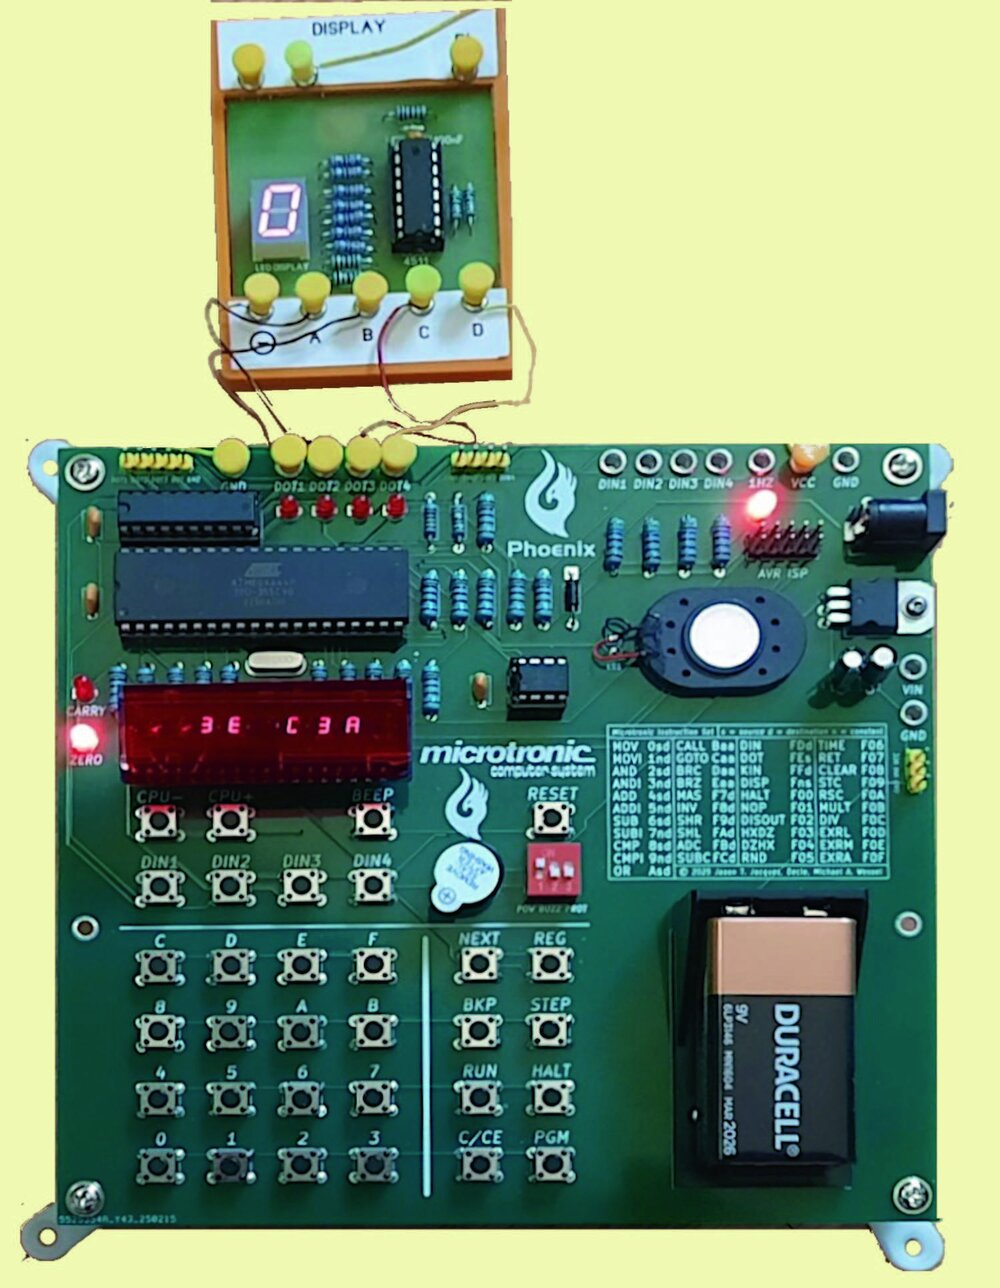
\includegraphics[keepaspectratio,alt={The Microtronic Phoenix, running the original firmware}]{images/phoenix.jpg}}

\emph{Figure 7. A new build running the original firmware: the
Microtronic Phoenix {[}16{]}.}

All Microtronic emulators published up to 2025 are complete
re-implementations: the Microtronic\textquotesingle s behavior
(operating system and virtual machine language) is emulated as
faithfully as possible by a program. Using the \emph{original}
Microtronic firmware was, until recently, impossible --- because it
simply was not available. Regrettably, neither Busch nor TI had archived
the Microtronic ROM, and the source code, too, had been lost; 40 years
after the project\textquotesingle s completion, no one could be located
at the MRT company either. Moreover, until then no procedure was known
that would allow the firmware ROM of a mask-programmed TMS1600 to be
read out: with a 6502- or Z80-based retro computer you can usually just
read the firmware (E)PROM with a programmer, but for the TMS1600 no
non-destructive procedure was known.

\subsubsection{Reading out the firmware}\label{reading-out-the-firmware}

This has now changed through our team\textquotesingle s work {[}17{]}.
In early 2024, on the occasion of a YouTube video about the "Radio Shack
Science Fair Microcomputer Trainer" (SFMT), the author was contacted by
Jason T. Jacques and "Decle", who had successfully read out the ROM of
that very SFMT. The SFMT uses the "little brother" of the TMS1600 ---
the TMS1100. Might it therefore be possible to read the Microtronic
firmware with the same method? It was not quite that simple. But over
the following months our team developed a procedure that ultimately
yielded the read-out Microtronic ROM. For this, the TMS1600 --- like the
TMS1100 before it --- had to be put into its so-called test mode. The
details of the TMS1600 test mode were not known, and there was no
documented case on the internet; our experiments first had to determine
which TMS1600 I/O pins activate this mode on reset. We also found that
the protocol for serially (bit-by-bit) reading the ROM differs markedly
from the documented TMS1100 protocol. This Microtronic-ROM "archaeology"
thus required several weeks of intensive work and extensive
experimentation. Despite all efforts, a few bits in the ROM image
remained ambiguous, because the read-out process was not 100\%
deterministic; these were corrected manually by Jason through extensive
firmware analysis and "sharp thinking", using "Decle"\textquotesingle s
TMS1600 disassembler (he had also previously built the Arduino-based
hardware and software for reading the SFMT\textquotesingle s TMS1xxx
firmware).

\subsubsection{The Phoenix}\label{the-phoenix}

The Microtronic ROM is interesting not only as a historical document, or
for fully understanding the Microtronic\textquotesingle s internals ---
we wanted to see it running again, on new hardware. That was also the
only way to verify that we had indeed read out a working, authentic ROM
(the read-out being somewhat "fuzzy"). So we built the
Microtronic\textquotesingle s software brain a new body --- the
\href{https://github.com/lambdamikel/microtronic-phoenix}{\textbf{Microtronic
Phoenix}} {[}16{]}. It has been flying again since February 2025 and is
made available to the public for replication. It is an ATmega-based
hardware emulator that runs the original Microtronic ROM by means of a
TMS1600 emulator {[}18{]}.

As soon as the firmware was available, in autumn 2024, Jason had already
rebuilt the Microtronic on a breadboard using the original hardware
components (even an external 2114 SRAM). That prototype used shift
registers to multiply the ports, which slowed the emulation, so in early
2025 we switched to the larger ATmega 644: it has enough I/O pins, more
program memory and SRAM, and can be clocked with an external 20 MHz
crystal. The Phoenix essentially gets by with a single chip --- the
ATmega 644 --- though we added an external 256 kbit EEPROM as "mass
storage" for programs, and a 74LS244 to decouple/protect the ATmega
pins, which are brought out directly as the Microtronic I/O ports for
experiments with Busch kits (or breadboards); in case of mishap,
replacing a 74LS244 is cheaper than the ATmega. The EEPROM has room for
42 complete Microtronic memory dumps. The result behaves absolutely
identically to the original --- it runs the same firmware. A more
authentic emulation is not possible: since we cannot simply program a
"new" TMS1600 with the Microtronic firmware, TMS1600 emulation (here in
hardware) remains the only way to let the original firmware fly again. A
piezo buzzer is also on board, connectable via a DIP switch to
Microtronic output 4 (for experiments needing tone); four extra keys,
DIN1--DIN4, can tie the corresponding Microtronic inputs HIGH (the
original has two console buttons "G" and "H" often wired to inputs as
external controls).

\subsubsection{The Neo firmware}\label{the-neo-firmware}

In addition to the original Microtronic mode, the Phoenix has a second
firmware --- a further development of the earlier Arduino emulators: the
\textbf{"Neo" firmware}. On power-up/reset the Phoenix asks which to use
("1" for Neo, "2" for Phoenix). Neo offers extras --- e.g. the
loudspeaker can produce tones via redundant Microtronic instructions (as
for PicoRAM), so simple melodies and sound effects can be programmed ---
and it is up to three times faster.

Neo also gives access to the EEPROM. On the original, PGM 1/PGM 2 access
the 2095 cassette interface to load/save programs; we did not rebuild
the cassette interface (the Phoenix cannot generate the 32 kHz tone
clock the 2095 needs, although it runs the same PGM 1/PGM 2 ROM routines
--- but the
\href{https://github.com/lambdamikel/microtronic-2095-arduino-emulator}{2095
SD-card emulator} {[}15{]} can be used). More practical is to use PGM
1/PGM 2 in Neo mode to access the EEPROM, loading/saving a full memory
image via "slot" numbers 0--41 as "program names" (back in the day one
noted the cassette counter reading instead). But how can the Phoenix
firmware access the EEPROM, given the original ROM has no such code? A
trick: the active firmware can be switched at any time by pressing
reset, and both modes always see the same memory contents --- so a
program can be loaded from EEPROM under Neo and then switched to Phoenix
mode, and run in either. This is handy for development too: develop in
Phoenix mode and switch to Neo for speed, or develop in Neo (more direct
EEPROM access) and switch to Phoenix for the most authentic behavior. A
further advantage of Neo is that the virtual machine language (or the
redundant instructions) can easily be adapted for one\textquotesingle s
own experiments --- it is, after all, a simple Arduino "C" program (not
so easy with the original firmware). Thus a Microtronic variant was
developed that acts as a MIDI drum computer / "drum sequencer",
requiring extensive instruction-set extensions and machine-language
changes; this "Microtronic drum computer" won a prize in the
RetroChallenge RC 2021/10 {[}19{]}.

Despite all these extensions and advantages, nothing will be dearer to
the Microtronic fan than the original. With the Phoenix we now have,
after 44 years, a re-edition of the Microtronic that truly deserves the
name: an emulator that could not be more authentic. The name
\emph{Phoenix} therefore seemed fitting --- the Microtronic ROM, all but
lost in the flames of history, flies once more, and with it the
Microtronic. With new hardware the Microtronic has now truly become
"immortal", and will go on finding new fans for decades to come.

\end{document}
